\section{Erstellung eines Modells zur Bodenatmung}
\label{sec-model}

Der Datensatz enthält sehr viele Features im Vergleich zur Anzahl an Messungen. Der Suchraum der Variablenselektion wäre viel zu groß.

\subsubsection{Test auf Vorliegen einer Normalverteilung}

Es werden nur normalverteilte (\it{Shapiro-Wilk}) und stark korrelierende (\it{Pearson}) Variablen in Betracht gezogen. Um \it{Pearson} als Korrelationskoeffizienten nutzen zu können, müssen die Messungen der Variablen normalverteilt sein. Um dies zu testen nutzen wir den \it{Shapiro-Wilk-Test}. Wenn die \it{p-Value} des \it{Shapiro-Wilk-Test} kleiner als $0.05$ ist, dann ist die Variable normalverteilt. Wir in Abbildung \ref{fig:shapiro} zu sehen ist, sind nur 14 der insgesamt 33 Variablen normalverteilt.

\begin{figure}[ht]
	\centering
	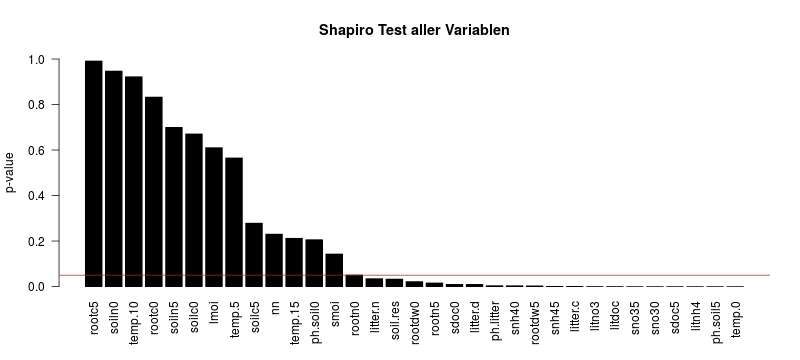
\includegraphics[width=\textwidth]{fig/model/normalverteilung-shapiro.png}
	\caption{\it{P-Value} des \bf{Shapiro-Wilk-Test} aller Variablen.}
	\label{fig:shapiro}
\end{figure}

\subsection{Korrelationsanalyse}

Aus den normalverteilten Variablen werden die am stärksten korrelierenden Variablen ausgewählt (siehe Abbildung \ref{fig:pearson}). 

\begin{figure}
	\centering
	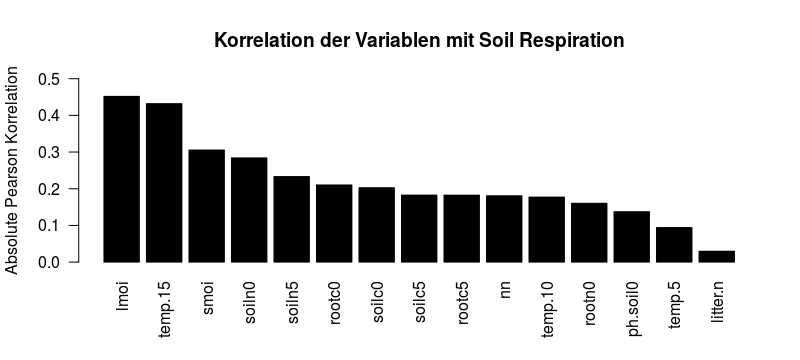
\includegraphics[width=\textwidth]{fig/model/correlation-pearson-normal.png}
	\caption{\bf{Pearson-Korrelation} der normalverteilten Einflussgrößen (\it{p-Value} $> 0.32$) mit der Bodenatmung.}
    \label{fig:pearson}
\end{figure}

\begin{itemize}
\tightlist
\item
  \emph{lmoi} relative Feuchte der Streuschicht (litter moisture)
\item
  \emph{temp15} Bodentemperatur in 15 cm Tiefe
\item
  \emph{smoi} relative Bodenfeuchte (soil moisture)
\item
  \emph{soiln0} Stickstoffgehalt des Bodens in 0-5 cm Tiefe
\end{itemize}

\subsection{Transformationen}

Transformationen bringen keine deutlichen Verbesserungen der Variablen. Für diese Analyse wurde ein Scatterplot genutzt (Abbildung im Anhang).

\subsection{Variablenselektion}

Mit Hilfe des R-Pakets \emph{leaps} wird das Modell mit dem geringsten $BIC$ ausgewählt, welches das Kriterium der Modellqualität erfüllt.

\subsection{Ergebnis}
Qualität des gewählten Modells

\subsection{Umsetzung mit R}

\begin{lstlisting}
# Test auf Normalverteilung
hainich.shapiro <- mapply(function(x) shapiro.test(x)$p.value,hainich)
hainich.shapiro.ordered <- hainich.shapiro[order(hainich.shapiro, decreasing = T)]
barplot(hainich.shapiro.ordered, las = 2, ylim = c(0,1), col = "black",
        ylab = "p-value", main = "Shapiro Test aller Variablen")
abline(h=0.05, col="red")

hainich.normal <- hainich[names(hainich.shapiro.ordered[hainich.shapiro.ordered > 0.032])]

# Korrelation mit Pearson
hainich.pear <- abs(cor(hainich.normal))["soil.res",-16]
hainich.pear.ordered <- hainich.pear[order(hainich.pear, decreasing = T)]
barplot(hainich.pear.ordered, las = 2, ylim = c(0,0.5), col = "black",
        ylab = "Absolute Pearson Korrelation", main = "Korrelation der Variablen mit Soil Respiration")
\end{lstlisting}
